\section{Current Achievement}

이전 장에서 기술한 구현 내용으로 실험을 진행하였고, 이에 대한 결과는 그림 \ref{fig:current}에서 확인할 수 있다.
하지만 그림 \ref{fig:current}을 자세히 보면, 첫 번째 이미지 같은 경우, 사람이 전체적으로 초록색과 검은색으로 색칠되었음을 확인할 수 있다.
하지만 목표 스타일 이미지를 보면, 옷은 조금 더 초록색으로, 다리는 살색으로, 얼굴은 살색, 머리는 노란색으로 색칠이 되는 게 현실적이고 자연스러운 스타일 적용이라고 볼 수 있다.
이는 현재 모델의 style extractor가 224 x 224 크기의 이미지를 input으로 받고, 현재 구현된 모델은 주어진 이미지의 중심을 기준으로 224 x 224 이미지로 잘라서 넣었기 때문에, 모델 입장에서는 스타일 이미지의 가운데 부분 (그림 \ref{fig:center}) 만 볼 수 있게 된다. 직관적으로도 이는 전체적은 스타일 적용에 방해가 될 것으로 생각이 되고, 앞으로 개선해야할 문제점이라고 인식하였다.

또한, 그림 \ref{fig:current}의 두 번째, 세 번째 그림을 보면, 스케치의 배경은 단색이지만, 채색된 결과를 보면, 배경에 대해서는 불필요한 노이즈들이 채색되는 것을 확인할 수 있다.
따라서 우리는 이러한 부분도, 노이즈가 없는 깔끔한 배경으로 색칠이 되게 해야할 필요성을 느꼈다.
\begin{figure}[t]
	\centering
	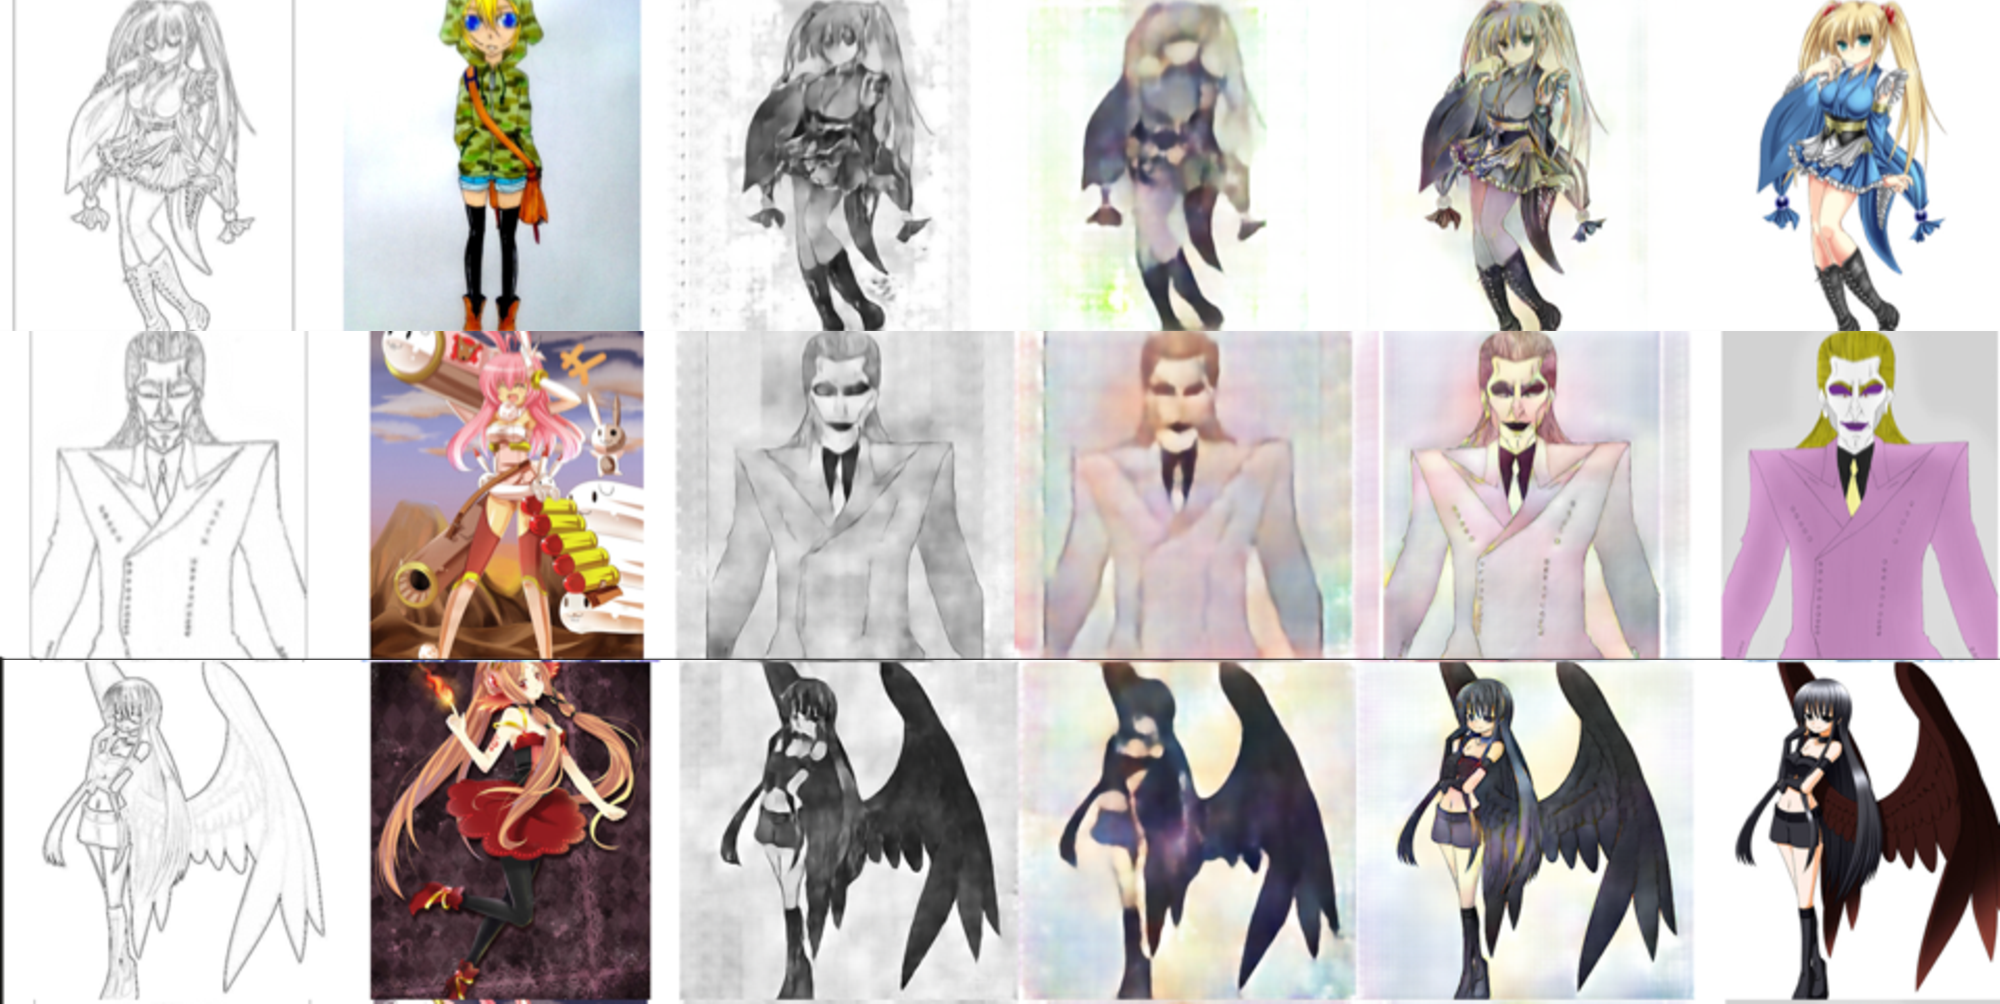
\includegraphics[width=\textwidth]{result}
	\caption{style2paint를 기반으로 한 모델 실험 결과. 가장 왼쪽부터, 주어진 스케치 이미지, 목표 스타일 이미지, Guide Decoder1의 결과, Guide Decoder2의 결과, 채색 결과, 원래 이미지이다.}
	\label{fig:current}
\end{figure}

\begin{figure}[t]
	\centering
	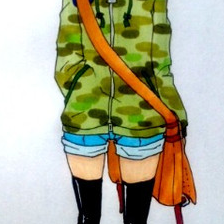
\includegraphics[width=0.2\textwidth]{center}
	\caption{그림 \ref{fig:current}의 첫 번째 스타일 이미지에서, 이미지의 중심을 기준으로 224 x 224 크기로 자른 부분. 현재 style extractor는 이 부분만 참고한다.}
	\label{fig:center}
\end{figure}

